\section{Deep Learning}

\begin{frame}[fragile]
  \frametitle{Introduction}
  \begin{itemize}
  \item What is Deep Learning?\\
  Deep Learning is a subfield of machine learning concerned with algorithms inspired by the structure and function of the brain called artificial neural networks.
  \item What is it used for?
  \begin{itemize}
  \item Self driving cars
  \item Beating humans in games
  \item Detecting spam in mails
  \item Forcasting stock prices
  \item Recognizing images in a picture
  \item Diagnosing illness (sometimes with better precision than doctors)
  \end{itemize}
  \end{itemize}
\end{frame}

\begin{frame}[fragile]
  \frametitle{University}
  Entry process for an university:
  \begin{itemize}
  \item Oral exam ($x_1$ value)
  \item Written exam ($x_2$ value)
  \end{itemize}
  Entry into the university is granted or denied based on $x_1$ and $x_2$.\\
  \vspace{3mm}
  
\includegraphics[scale=0.2]{img/stanford}
\end{frame}

\begin{frame}[fragile]
  \frametitle{University}
  Historical data: Green dots are accepted, red dots are rejected\\
  \vspace{3mm}
  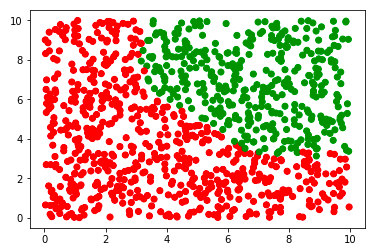
\includegraphics[scale=0.4]{img/uni_data}\\
  \vspace{3mm}
  \begin{exercise}
  Will a student with $x_1=5$ and $x_2=4$ be accepted?
  \end{exercise}
\end{frame}

\begin{frame}[fragile]
  \frametitle{University}
  Deep Learning will now be used to find the line between the red and the green dots.
  The line is the model!\\
  \vspace{3mm}
  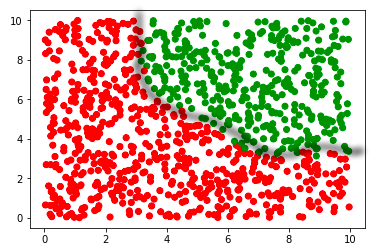
\includegraphics[scale=0.4]{img/uni_data_1}
\end{frame}

\begin{frame}[fragile]
  \frametitle{University}
  To start with a easier example, we assume that the line is a straight line.\\
  \vspace{3mm}
  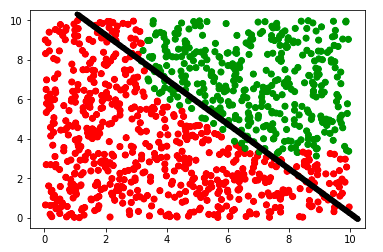
\includegraphics[scale=0.4]{img/uni_data_2}\\
  \vspace{3mm}
  What is the mathematical term for this line?\\
  $f(x)=mx+b$, or $ax_1+bx_2+c=0$\\
  \begin{exercise}
  What is the equation for the line in the picture?
  \end{exercise} 
\end{frame}

\begin{frame}[fragile]
  \frametitle{University}
  Two points could be taken on the line:\\
  $P_1: x_1=8, x_2=2.7$\\
  $P_2: x_1=3, x_2=8$\\
  \vspace{3mm}
  The line in the picture is: $1.06x_1+x_2-11.18=0$\\
  \vspace{3mm}
  Prediction:\\
  $Score > 0: Accept$ (above the line)\\
  $Score < 0: Reject$ (below the line)
\end{frame}

\begin{frame}[fragile]
  \frametitle{University}
  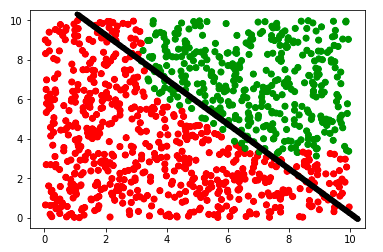
\includegraphics[scale=0.4]{img/uni_data_2}\\
  \vspace{3mm}
  $w_1x_1+w_2x_2+b=0$\\
  $Wx + b = 0$ (Vector Notation)\\
  $W = (w_1, w_2)$\\
  $x = (x_1, x_2)$\\
  W: Weights, x: Input, b: Bias\\
  $y$: Label: 0 (rejected) or 1 (accepted)\\
  \vspace{3mm}
  Prediction:
  $
  \hat{y}=\begin{cases}
    1, & \text{if $Wx+b \geq 0$}.\\
    0, & \text{if $Wx+b < 0$}.
  \end{cases}
  $  
\end{frame}

\begin{frame}[fragile]
  \frametitle{N Dimensions}
  If we have as input n dimensions, the equation will be the same:\\
  $w_1x_1+w_2x_2+\ldots+x_2x_n+b=0$\\
  $Wx + b = 0$\\
  $W = (w_1, w_2, \ldots, w_n)$\\
  $x = (x_1, x_2, \ldots, x_n)$\\
  W: Weights, x: Input, b: Bias\\
  $y$: Label: 0 (rejected) or 1 (accepted)\\
  \vspace{3mm}
  Prediction:
  $
  \hat{y}=\begin{cases}
    1, & \text{if $Wx+b \geq 0$}.\\
    0, & \text{if $Wx+b < 0$}.
  \end{cases}
  $  
\end{frame}

\begin{frame}[fragile]
  \frametitle{Peceptron}
  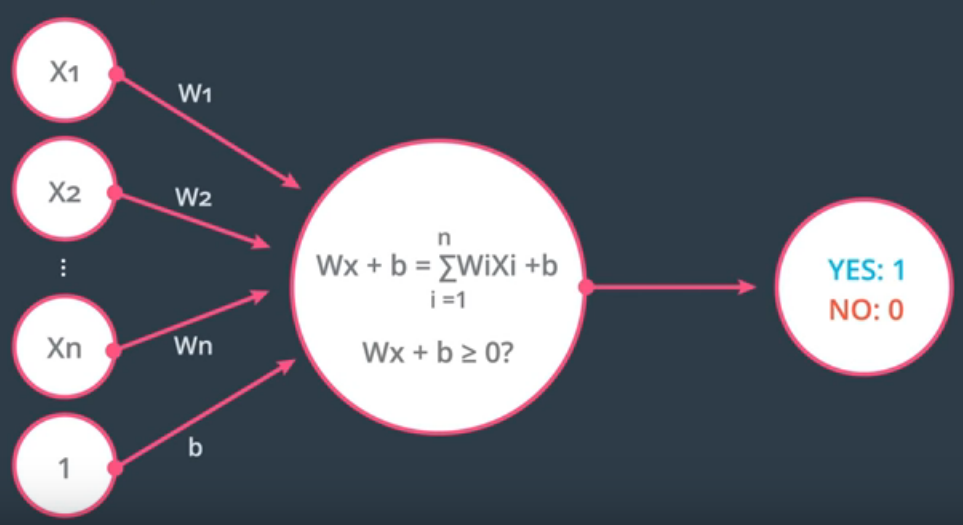
\includegraphics[scale=0.3]{img/perceptron}
\end{frame}

\begin{frame}[fragile]
  \frametitle{Step Function}
  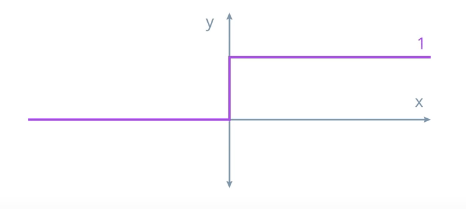
\includegraphics[scale=0.3]{img/stepfunction}\\
  \vspace{3mm}
  $
  y=\begin{cases}
    1, & \text{if $x \geq 0$}.\\
    0, & \text{if $x < 0$}.
  \end{cases}
  $
\end{frame}

\begin{frame}[fragile]
  \frametitle{Step Function}
  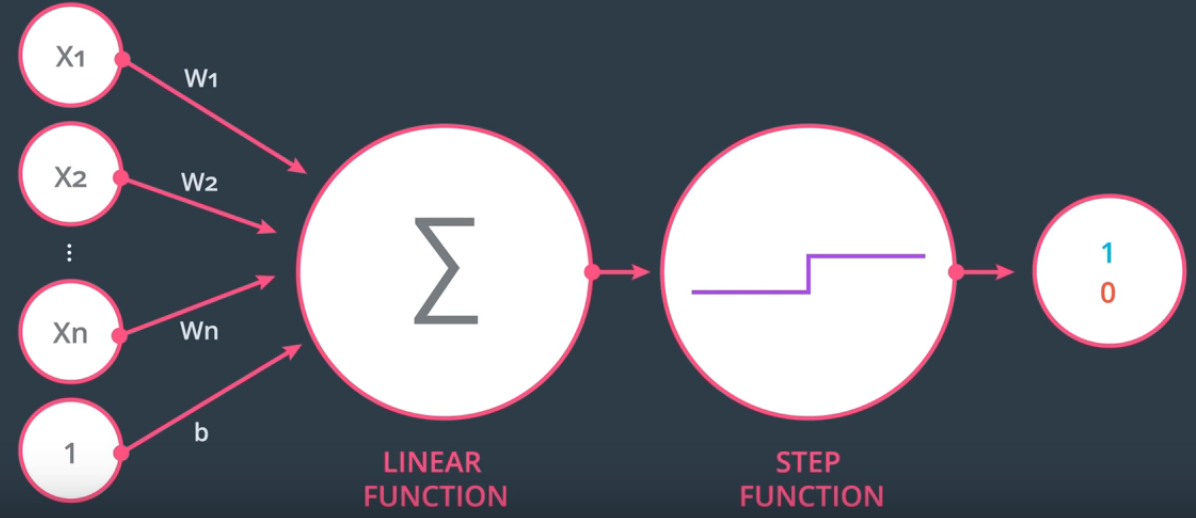
\includegraphics[scale=0.25]{img/perceptron_step}\\
  \vspace{3mm}
  Other functions (instead of the step function) could be used!
\end{frame}

\begin{frame}[fragile]
  \frametitle{Univerity}
  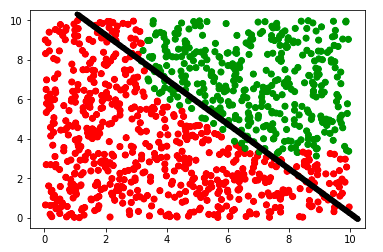
\includegraphics[scale=0.4]{img/uni_data_2}\\
  \vspace{3mm}
  How do we find the line between the green and red points?
\end{frame}

\begin{frame}[fragile]
  \frametitle{Univerity}
  Let's start with a simple example. The computer will draw a random line.\\
  \vspace{3mm}
  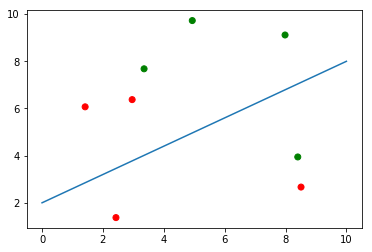
\includegraphics[scale=0.4]{img/uni_data_3}\\
  \vspace{3mm}
  How good or bad is this line? How many points are misclassified? Which points
  should be used to improve the line?
\end{frame}

\begin{frame}[fragile]
  \frametitle{Univerity}
  For each misclassified point, we need the line to come closer to the point!\\
  \vspace{3mm}
  Algorithm:\\
  For every misclassified point ($x_1...x_n$):\\
  \vspace{2mm}
  $\quad if \; prediction = 0:$\\
  $\qquad for \; i=1..n:$\\
  $\qquad \quad w_i = w_i + \alpha x_i$\\
  $\qquad b = b + \alpha$\\
  \vspace{2mm}
  $\quad if \; prediction = 1:$\\
  $\qquad for \; i=1..n:$\\
  $\qquad \quad w_i = w_i - \alpha x_i$\\
  $\qquad b = b - \alpha$
\end{frame}

\begin{frame}[fragile]
  \frametitle{Univerity}
  After repeating the algorithm for a 1000 times, we have the following result:\\
  \vspace{3mm}
  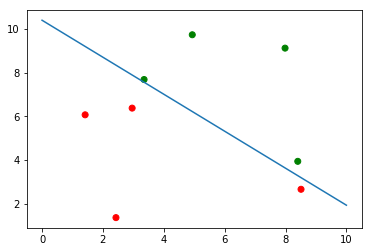
\includegraphics[scale=0.4]{img/uni_data_4}
\end{frame}

\begin{frame}[fragile]
  \frametitle{University}
  Now we know how to find a line. But if the solution is a curve, we need to adapt our
  algorithm. For that we are going to introduce the error function. With the error
  function, we have an idea how bad/good our line is.\\
  \vspace{3mm}
  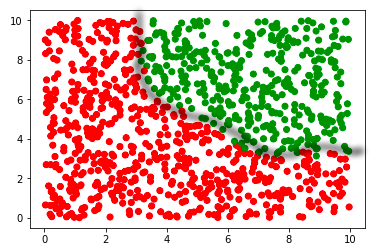
\includegraphics[scale=0.4]{img/uni_data_1}\\
  \vspace{3mm}
\end{frame}

\begin{frame}[fragile]
  \frametitle{Univerity}
  What could be the error function in the following picture? Could it be the number
  of misclassified points?\\
  \vspace{3mm}
  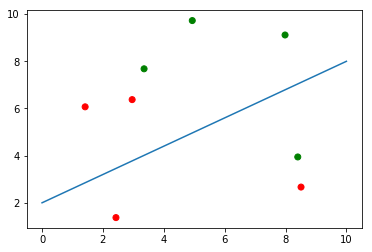
\includegraphics[scale=0.25]{img/error_1}
  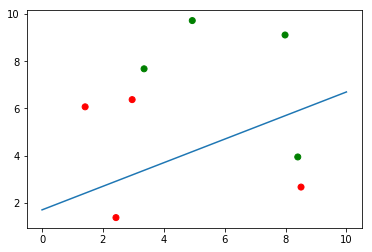
\includegraphics[scale=0.25]{img/error_2}
  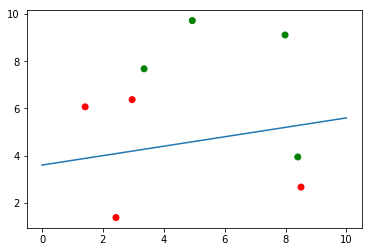
\includegraphics[scale=0.25]{img/error_3}\\
  \vspace{3mm}
  We do not know how to improve the line, as if we move it into different
  directions, the error (3 misclassified points) will be the same. We need
  something which tells us if the line is better or worse!\\
  In this case, the error function is discrete. But we need an error function
  which is continuous.
\end{frame}

